\documentclass[UTF8]{ctexart}
\usepackage{amsmath}   
\usepackage{booktabs}  
\usepackage{geometry}  
\usepackage{hyperref}
\usepackage{graphicx} 
\usepackage{float}
\graphicspath{{figure/}} % 指定放置图片的子文件夹路径
\geometry{a4paper, left=2.5cm, right=2.5cm, top=2.5cm, bottom=2.5cm}

\begin{document}

\title{计算流体力学第二次作业}
\author{朱林-2200011028}
\date{\today}
\maketitle

\section{数理算法原理}

\subsection{对于一阶导数$\frac{\partial u}{\partial x}$的差分格式}

\subsubsection{采用两个网格点的一阶格式}
利用泰勒展开式,对于$u_{i+1}$,我们有:
\begin{equation}
    u_{i+1} = u_i + \Delta x \frac{\partial u}{\partial x} + O(\Delta x^2)
\end{equation}
在等式两侧同时除以$\Delta x$,我们可以得到:
\begin{equation}
    \frac{u_{i+1} - u_i}{\Delta x} = \frac{\partial u}{\partial x} + O(\Delta x)
\end{equation}
由此可知,差分格式为:
\begin{equation}
    \frac{\partial u}{\partial x} = \frac{u_{i+1} - u_i}{\Delta x} 
\end{equation}
将右侧展开后观察阶数:
\begin{equation}
    \begin{aligned}
        \frac{u_{i+1} - u_i}{\Delta x} &= \frac{u_i + \Delta x \frac{\partial u}{\partial x} +  \frac{\Delta x^2}{2} \frac{\partial^2 u}{\partial x^2} + O(\Delta x^3) - u_i}{\Delta x} \\
        &= \frac{\Delta x \frac{\partial u}{\partial x} +  \frac{\Delta x^2}{2} \frac{\partial^2 u}{\partial x^2} + O(\Delta x^3)}{\Delta x} \\
        &= \frac{\partial u}{\partial x} + \frac{\Delta x}{2} \frac{\partial^2 u}{\partial x^2} + O(\Delta x^2)
    \end{aligned}
\end{equation}
由于截断误差为一阶,所以,该格式为一阶格式。

\subsubsection{采用四个网格点的三阶格式}
采用待定系数法,我们采用四个网格点来构造差分格式,设这一格式为:
\begin{equation}
   \frac{\partial u}{\partial x} = a_1 u_{i-1} + a_2 u_i + a_3 u_{i+1} + a_4 u_{i+2}
\end{equation}
将$u_{i-1}$、、$u_{i+1}$、$u_{i+2}$分别用泰勒展开式展开,得到:
\begin{equation}
    \begin{aligned}
        u_{i-1} &= u_i - \Delta x \frac{\partial u}{\partial x} + \frac{(\Delta x)^2}{2} \frac{\partial^2 u}{\partial x^2} - \frac{(\Delta x)^3}{6} \frac{\partial^3 u}{\partial x^3} + O(\Delta x^4) \\
        u_{i+1} &= u_i + \Delta x \frac{\partial u}{\partial x} + \frac{(\Delta x)^2}{2} \frac{\partial^2 u}{\partial x^2} + \frac{(\Delta x)^3}{6} \frac{\partial^3 u}{\partial x^3} + O(\Delta x^4) \\
        u_{i+2} &= u_i + 2\Delta x \frac{\partial u}{\partial x} + 2(\Delta x)^2 \frac{\partial^2 u}{\partial x^2} + \frac{4(\Delta x)^3}{3} \frac{\partial^3 u}{\partial x^3} + O(\Delta x^4)
    \end{aligned}
\end{equation}
带入(4)式中,得到:
\begin{equation}
    \begin{aligned}
        \frac{\partial u}{\partial x} &= a_1 \left( u_i - \Delta x \frac{\partial u}{\partial x} + \frac{(\Delta x)^2}{2} \frac{\partial^2 u}{\partial x^2} - \frac{(\Delta x)^3}{6} \frac{\partial^3 u}{\partial x^3} + O(\Delta x^4) \right) + a_2 u_i \\
        &+ a_3 \left( u_i + \Delta x \frac{\partial u}{\partial x} + \frac{(\Delta x)^2}{2} \frac{\partial^2 u}{\partial x^2} + \frac{(\Delta x)^3}{6} \frac{\partial^3 u}{\partial x^3} + O(\Delta x^4) \right) \\
        &+ a_4 \left( u_i + 2\Delta x \frac{\partial u}{\partial x} + 2(\Delta x)^2 \frac{\partial^2 u}{\partial x^2} + \frac{4(\Delta x)^3}{3} \frac{\partial^3 u}{\partial x^3} + O(\Delta x^4) \right)\\
        &= (a_1 + a_2 + a_3 + a_4) u_i + \left( -a_1 + a_3 + 2a_4 \right) \Delta x \frac{\partial u}{\partial x} + \left( \frac{a_1}{2} + \frac{a_2}{2} + a_3 + 2a_4 \right) (\Delta x)^2 \frac{\partial^2 u}{\partial x^2} \\
        &+ \left( -\frac{a_1}{6} + \frac{a_2}{6} + \frac{a_3}{6} + \frac{4a_4}{3} \right) (\Delta x)^3 \frac{\partial^3 u}{\partial x^3} + O(\Delta x^3)
    \end{aligned}
\end{equation}
比较两侧系数得到一下方程组:
\begin{equation}
    \begin{cases}
        a_1 + a_2 + a_3 + a_4 &= 0 \\
        \Delta x(-a_1 + a_3 + 2a_4) &= 1 \\
        \frac{a_1}{2} + \frac{a_3}{2} + 2a_4 &= 0 \\
        -\frac{a_1}{6} + \frac{a_3}{6} + \frac{4a_4}{3} &= 0
    \end{cases}
\end{equation}
解得:
\begin{equation}
    \begin{cases}
        a_1 &=  -\frac{1}{3\Delta x}\\
        a_2 &=  -\frac{1}{2\Delta x}\\
        a_3 &=  \frac{1}{\Delta x}\\
        a_4 &=  -\frac{1}{6\Delta x}
    \end{cases}
\end{equation}
因此,最终的四网格点差分格式为:
\begin{equation}
    \frac{\partial u}{\partial x} = \frac{-2u_{i-1}-3u_i + 6u_{i+1} - u_{i+2}}{6\Delta x} 
\end{equation}
为了分析差分格式$\frac{\partial u}{\partial x} = \frac{-2u_{i-1} - 3u_i + 6u_{i+1} - u_{i+2}}{6\Delta x}$的截断误差阶数,我们使用泰勒展开法,将各节点值在$u_i$处展开:
$$
\begin{aligned}
u_{i-1} &= u_i - \Delta x \frac{\partial u}{\partial x}\bigg|_i + \frac{\Delta x^2}{2} \frac{\partial^2 u}{\partial x^2}\bigg|_i - \frac{\Delta x^3}{6} \frac{\partial^3 u}{\partial x^3}\bigg|_i + \frac{\Delta x^4}{24} \frac{\partial^4 u}{\partial x^4}\bigg|_i + O(\Delta x^5), \\
u_{i+1} &= u_i + \Delta x \frac{\partial u}{\partial x}\bigg|_i + \frac{\Delta x^2}{2} \frac{\partial^2 u}{\partial x^2}\bigg|_i + \frac{\Delta x^3}{6} \frac{\partial^3 u}{\partial x^3}\bigg|_i + \frac{\Delta x^4}{24} \frac{\partial^4 u}{\partial x^4}\bigg|_i + O(\Delta x^5), \\
u_{i+2} &= u_i + 2\Delta x \frac{\partial u}{\partial x}\bigg|_i + 2\Delta x^2 \frac{\partial^2 u}{\partial x^2}\bigg|_i + \frac{4\Delta x^3}{3} \frac{\partial^3 u}{\partial x^3}\bigg|_i + \frac{2\Delta x^4}{3} \frac{\partial^4 u}{\partial x^4}\bigg|_i + O(\Delta x^5).
\end{aligned}
$$
代入分子表达式并合并同类项:
$$
\begin{aligned}
-2u_{i-1} &= -2u_i + 2\Delta x \frac{\partial u}{\partial x}\bigg|_i - \Delta x^2 \frac{\partial^2 u}{\partial x^2}\bigg|_i + \frac{\Delta x^3}{3} \frac{\partial^3 u}{\partial x^3}\bigg|_i - \frac{\Delta x^4}{12} \frac{\partial^4 u}{\partial x^4}\bigg|_i + \cdots, \\
6u_{i+1} &= 6u_i + 6\Delta x \frac{\partial u}{\partial x}\bigg|_i + 3\Delta x^2 \frac{\partial^2 u}{\partial x^2}\bigg|_i + \Delta x^3 \frac{\partial^3 u}{\partial x^3}\bigg|_i + \frac{\Delta x^4}{4} \frac{\partial^4 u}{\partial x^4}\bigg|_i + \cdots, \\
-u_{i+2} &= -u_i - 2\Delta x \frac{\partial u}{\partial x}\bigg|_i - 2\Delta x^2 \frac{\partial^2 u}{\partial x^2}\bigg|_i - \frac{4\Delta x^3}{3} \frac{\partial^3 u}{\partial x^3}\bigg|_i - \frac{2\Delta x^4}{3} \frac{\partial^4 u}{\partial x^4}\bigg|_i + \cdots.
\end{aligned}
$$
合并后:
$$
\small
\begin{aligned}
\text{分子} &= \left(6\Delta x \frac{\partial u}{\partial x}\bigg|_i \right) + \left(-\frac{1}{2}\Delta x^4 \frac{\partial^4 u}{\partial x^4}\bigg|_i \right) + O(\Delta x^5)
\end{aligned}
$$
除以$6\Delta x$后得到:
$$
\frac{\partial u}{\partial x}\bigg|_i - \frac{1}{12}\Delta x^3 \frac{\partial^4 u}{\partial x^4}\bigg|_i + O(\Delta x^4)
$$
截断误差的主项为$\,-\frac{1}{12}\Delta x^3 \frac{\partial^4 u}{\partial x^4}\bigg|_i$,故截断误差是三阶的。


\subsection{对于二阶导数$\frac{\partial^2 u}{\partial x^2}$的差分格式}

\subsubsection{采用三个网格点的一阶格式}
利用泰勒展开式,对于$u_{i+1}$,我们有:
\begin{equation}
    u_{i+1} = u_i + \Delta x \frac{\partial u}{\partial x} + \frac{\Delta x^2}{2} \frac{\partial^2 u}{\partial x^2} + O(\Delta x^3)
\end{equation}
对于$u_{i+2}$,我们有:
\begin{equation}
    u_{i+2} = u_i + 2\Delta x \frac{\partial u}{\partial x} + 2(\Delta x)^2 \frac{\partial^2 u}{\partial x^2} + O(\Delta x^3)
\end{equation}
利用(10)式和(11)式,消去$\frac{\partial u}{\partial x}$,我们可以得到该差分公式:
\begin{equation}
    \frac{\partial^2 u}{\partial x^2} = \frac{u_{i+2} - 2u_{i+1} + u_i}{(\Delta x)^2}
\end{equation}
将右侧展开后观察阶数:
\begin{equation}
    \begin{aligned}
        \frac{u_{i+2} - 2u_{i+1} + u_i}{(\Delta x)^2} &= \frac{1}{(\Delta x)^2}\cdot [(u_i + 2\Delta x \frac{\partial u}{\partial x} + 2(\Delta x)^2 \frac{\partial^2 u}{\partial x^2} + \frac{4(\Delta x)^3}{3} \frac{\partial^3 u}{\partial x^3} + O(\Delta x^4)) \\
        &- 2(u_i + \Delta x \frac{\partial u}{\partial x} + \frac{(\Delta x)^2}{2} \frac{\partial^2 u}{\partial x^2} + \frac{(\Delta x)^3}{6} \frac{\partial^3 u}{\partial x^3} + O(\Delta x^4)) + u_i] \\
        &= \frac{(\Delta x)^2\frac{\partial^2 u}{\partial x^2} + (\Delta x)^3 \frac{\partial^3 u}{\partial x^3} + O(\Delta x^4)}{(\Delta x)^2} \\
        &= \frac{\partial^2 u}{\partial x^2} + (\Delta x) \frac{\partial^3 u}{\partial x^3} + O(\Delta x^2)
    \end{aligned}
\end{equation}
因此,该格式为一阶格式。

\subsubsection{采用三个网格点的二阶格式}
同理,首先设定差分格式为:
\begin{equation}
    \frac{\partial^2 u}{\partial x^2} = b_1 u_{i-1} + b_2 u_i + b_3 u_{i+1}
\end{equation}
对于$u_{i-1}$、$u_{i+1}$,我们有:
\begin{equation}
    \begin{aligned}
        u_{i-1} &= u_i - \Delta x \frac{\partial u}{\partial x} + \frac{(\Delta x)^2}{2} \frac{\partial^2 u}{\partial x^2} - \frac{(\Delta x)^3}{6} \frac{\partial^3 u}{\partial x^3} + O(\Delta x^4) \\
        u_{i+1} &= u_i + \Delta x \frac{\partial u}{\partial x} + \frac{(\Delta x)^2}{2} \frac{\partial^2 u}{\partial x^2} + \frac{(\Delta x)^3}{6} \frac{\partial^3 u}{\partial x^3} + O(\Delta x^4)
    \end{aligned}
\end{equation}
带入得到:
\begin{equation}
    \begin{aligned}
        \frac{\partial^2 u}{\partial x^2} &= b_1 \left( u_i - \Delta x \frac{\partial u}{\partial x} + \frac{(\Delta x)^2}{2} \frac{\partial^2 u}{\partial x^2} - \frac{(\Delta x)^3}{6} \frac{\partial^3 u}{\partial x^3} + O(\Delta x^4) \right) \\
        &+ b_2 u_i + b_3 \left( u_i + \Delta x \frac{\partial u}{\partial x} + \frac{(\Delta x)^2}{2} \frac{\partial^2 u}{\partial x^2} + \frac{(\Delta x)^3}{6} \frac{\partial^3 u}{\partial x^3} + O(\Delta x^4) \right)\\
        &= (b_1 + b_2 + b_3) u_i + (-b_1 + b_3) \Delta x \frac{\partial u}{\partial x} + (\frac{b_1}{2} + \frac{b_3}{2}) (\Delta x)^2 \frac{\partial^2 u}{\partial x^2} \\
        &+ (-\frac{b_1}{6} + \frac{b_3}{6}) (\Delta x)^3 \frac{\partial^3 u}{\partial x^3} + O(\Delta x^2)
    \end{aligned}
\end{equation}
比较两侧系数得到以下方程组:
\begin{equation}
    \begin{cases}
        b_1 + b_2 + b_3 &= 0 \\
        -b_1 + b_3 &= 0 \\
        (\Delta x)^2 (\frac{b_1}{2} + \frac{b_3}{2}) &= 1 \\
        -\frac{b_1}{6} + \frac{b_3}{6} &= 0
    \end{cases}
\end{equation}
解得:
\begin{equation}
    \begin{cases}
        b_1 &=  \frac{1}{\Delta x^2}\\
        b_2 &=  -2\frac{1}{\Delta x^2}\\
        b_3 &=  \frac{1}{\Delta x^2}
    \end{cases}
\end{equation}
因此,最终的三网格点差分格式为:
\begin{equation}
    \frac{\partial^2 u}{\partial x^2} = \frac{u_{i-1} - 2u_i + u_{i+1}}{\Delta x^2}
\end{equation}
同理,将右侧展开后观察阶数可以得知该格式为二阶格式。


\section{代码生成与调试}
计算误差 $error$ 的思路为:
\begin{itemize}
    \item 定义一个已知解析解的函数,程序中采用的是三次函数$f_3(x) = x^3 - 2x^2 + 3x + 1$和三角函数$g(x) = \sin(kx)$
    \item 通过数值方法计算出该函数的一阶导数和二阶导数
    \item 通过解析解计算出该函数的一阶导数和二阶导数
    \item 计算数值解与解析解的误差
\end{itemize}
验证精度的思路为:
\begin{itemize}
    \item 通过不同的网格步长,计算出数值解
    \item 计算出不同网格下的误差
    \item 根据步长与误差的关系,
    \begin{equation}
        error = C \cdot \Delta x^p + O(\Delta x^{p+1}) + e
    \end{equation}
    其中,$C$为常数,$p$为阶数,$e$为舍入误差
    将步长与误差同时取对数,如果舍入误差可以忽略,则可以
    \begin{equation}
        \log(error) = \log(C) + p \cdot \log(\Delta x)
    \end{equation}
    通过线性拟合函数 $y = kx + b$,可以得到拟合
    函数的斜率$k$,与理论阶数$p$相比较,可以通过斜率来验证精度
\end{itemize}
与此同时,还修改了数据的存储精度,比较了单精度和双精度的计算结果。
具体的生成与调试参见github仓库:
\begin{center}
    \url{https://github.com/ZeroLevelKing/CFD_hw2.git}
\end{center}
git的commit记录如下:

\begin{figure}[H]
    \centering
    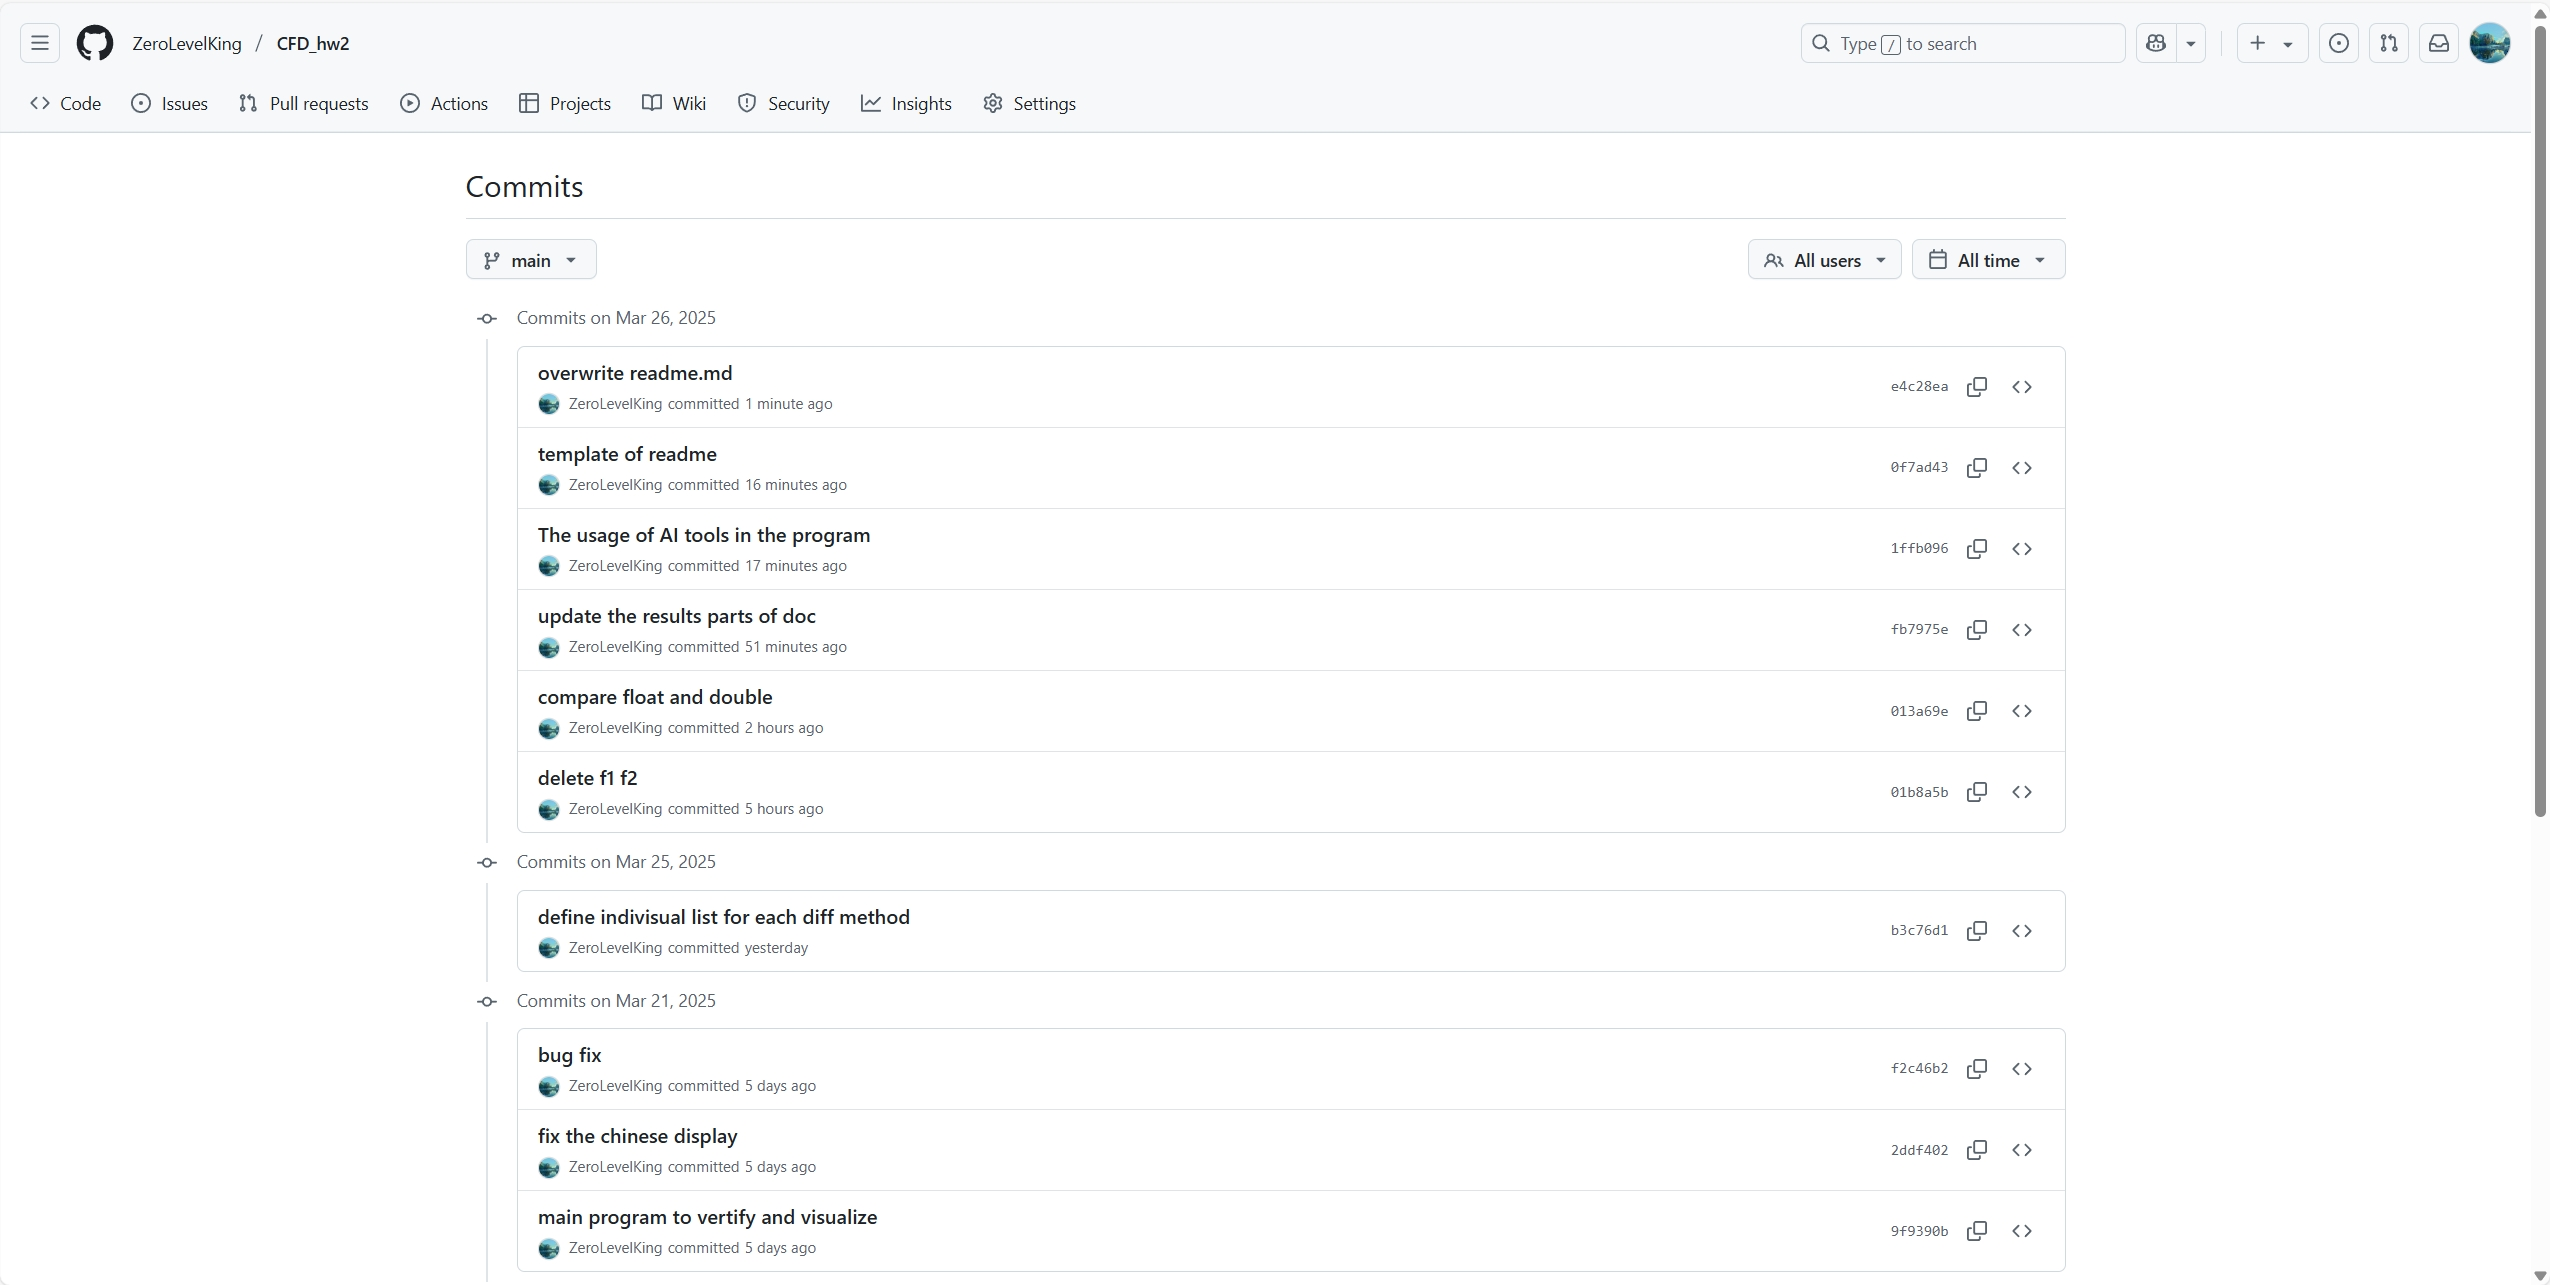
\includegraphics[width=0.8\textwidth]{c1.png} 
\end{figure}
\begin{figure}[H]
    \centering
    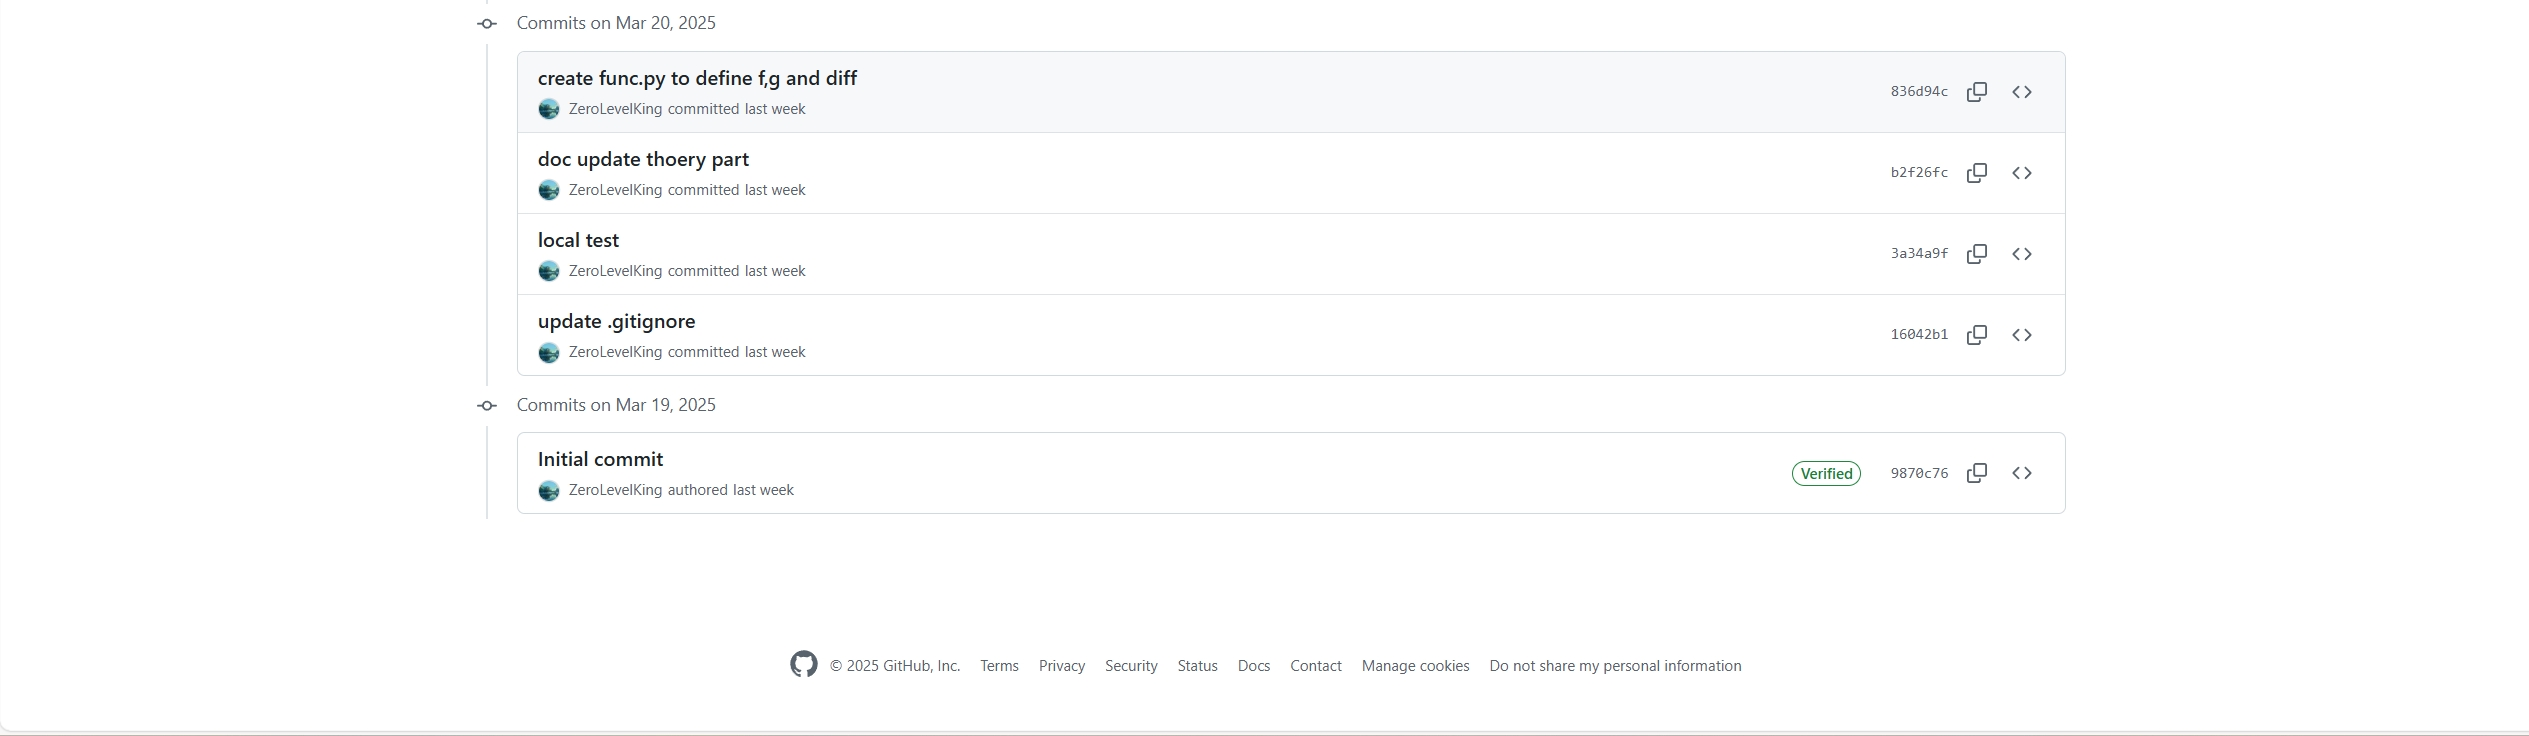
\includegraphics[width=0.8\textwidth]{c2.png} 
\end{figure}

\section{结果讨论和物理解释}
对于三次函数$f_3(x) = x^3 - 2x^2 + 3x + 1$和三角函数$g(x) = \sin(kx)$($k = 0.1$),
对于 $x = 1$ 处的导数和二阶导数,按照上述方法得到的数值解与解析解的误差以及拟合结果如下:

\begin{figure}[H]
    \centering
    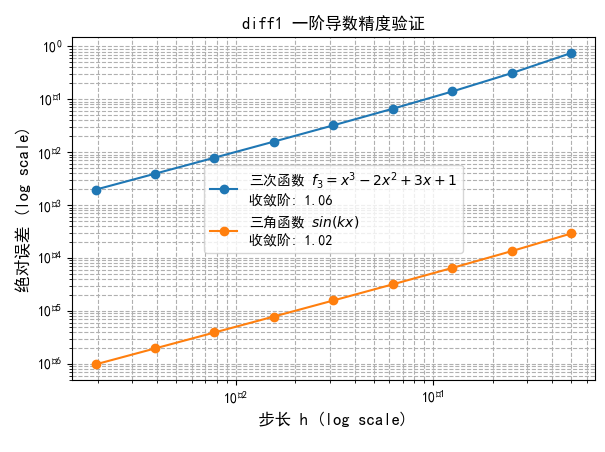
\includegraphics[width=0.8\textwidth]{f1.png} 
    \caption{差分格式 $\frac{\partial u}{\partial x} = \frac{u_{i+1} - u_i}{\Delta x}$ 的误差与拟合结果}
    \label{fig:result1} 
\end{figure}
\begin{figure}[H]
    \centering
    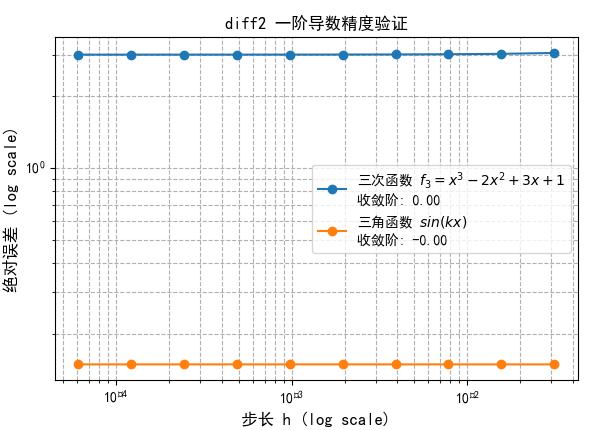
\includegraphics[width=0.8\textwidth]{f2.png} 
    \caption{差分格式 $\frac{\partial u}{\partial x} = \frac{-2u_{i-1}-3u_i + 6u_{i+1} - u_{i+2}}{6\Delta x}$  的误差与拟合结果}
    \label{fig:result2} 
\end{figure}
\begin{figure}[H]
    \centering
    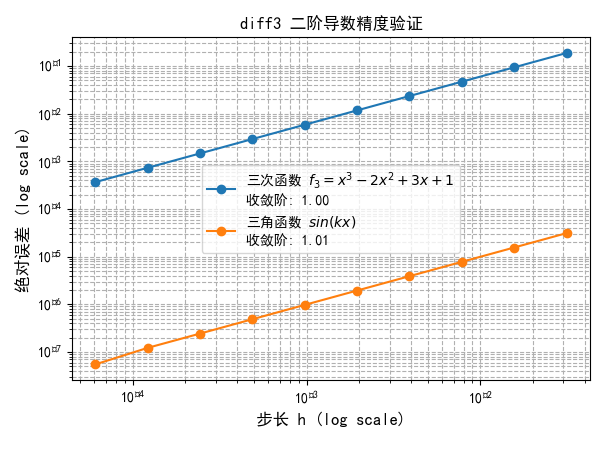
\includegraphics[width=0.8\textwidth]{f3.png} 
    \caption{差分格式 $\frac{\partial^2 u}{\partial x^2} = \frac{u_{i+2} - 2u_{i+1} + u_i}{(\Delta x)^2}$  的误差与拟合结果}
    \label{fig:result3} 
\end{figure}
\begin{figure}[H]
    \centering
    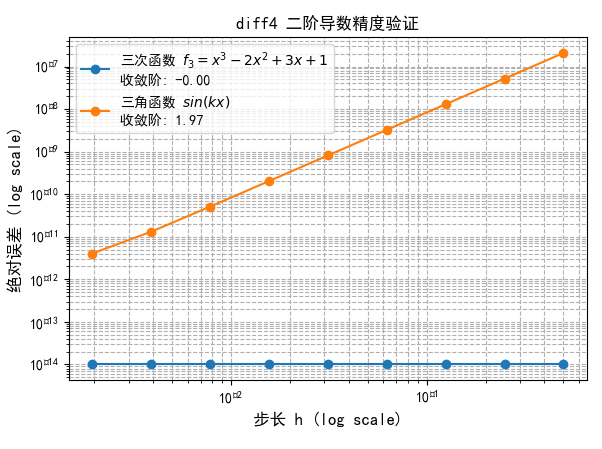
\includegraphics[width=0.8\textwidth]{f4.png} 
    \caption{差分格式 $\frac{\partial^2 u}{\partial x^2} = \frac{u_{i-1} - 2u_i + u_{i+1}}{\Delta x^2}$  的误差与拟合结果}
    \label{fig:result4} 
\end{figure}

\begin{itemize}
    \item 通过上述结果可以发现,对于第一种差分格式,可以很明显地观察到其误差与步长的一阶关系,
    \item 而对于第二种差分格式,理论上应该是三阶关系:对于三次函数,其没有截断误差,只有舍入误差,所以误差不随步长变化;对于三角函数,由于机器精度的限制,舍入误差占据主要因素,在步长较短时,几乎不随步长变化,导致斜率接近于0。
    \item 由图可知,第三种差分格式的收敛阶是1,与理论吻合很好
    \item 第四种差分格下:三次函数无截断误差,舍入误差占据主要因素,导致斜率接近于0;三角函数的收敛阶是2,与理论吻合很好
\end{itemize}

对于单精度和双精度对于结果的影响探究如下:
\begin{figure}[H]
    \centering
    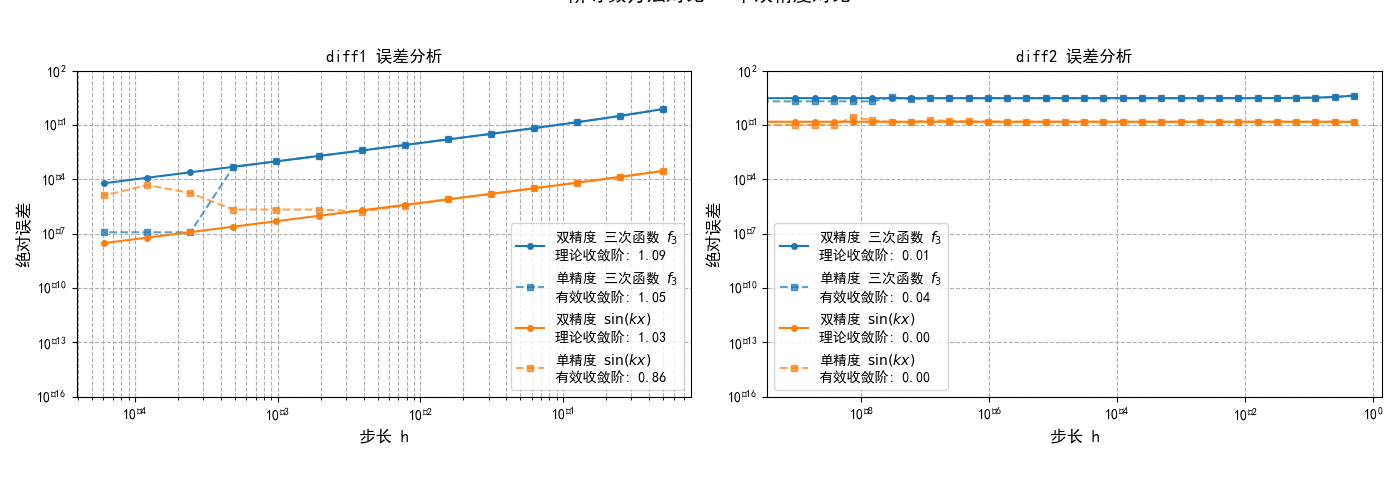
\includegraphics[width=0.8\textwidth]{Figure_3.png} 
    \caption{单精度和双精度对于一阶导数差分格式的影响}
\end{figure}
\begin{figure}[H]
    \centering
    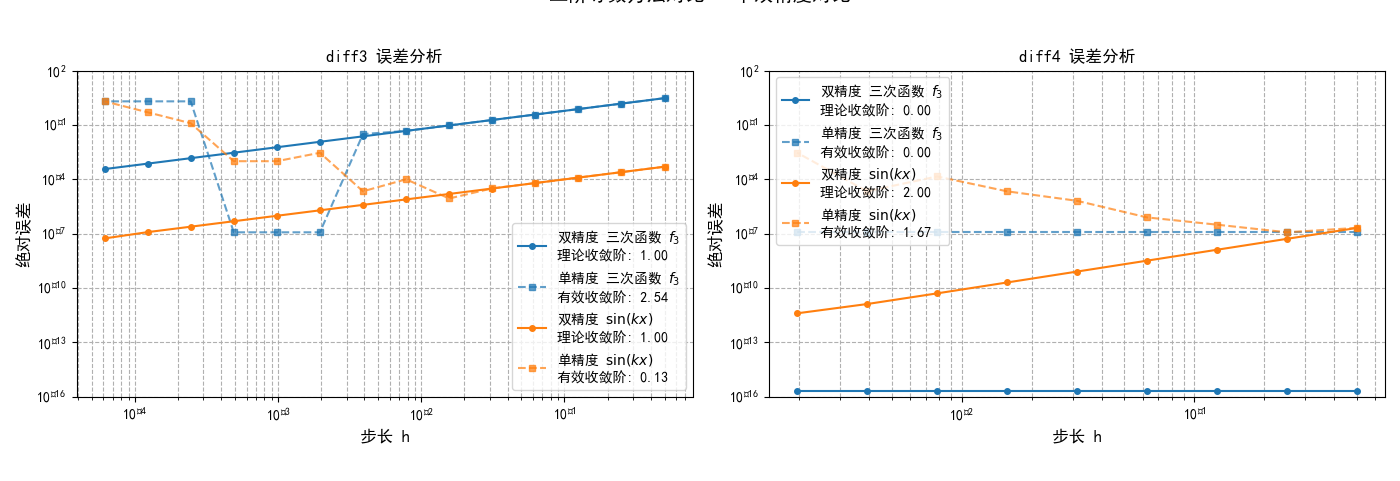
\includegraphics[width=0.8\textwidth]{Figure_4.png} 
    \caption{单精度和双精度对于二阶导数差分格式的影响}
\end{figure}

\begin{itemize}
    \item 可以看出,单精度和双精度的区别主要在步长较小时,舍入误差占据主要因素,单精度由于舍入误差更大,会导致结果偏离理论值。
    \item 而在步长较大时,单精度和双精度的结果几乎没有区别,说明此时的误差主要影响因素是截断误差。
\end{itemize}

%附录
\newpage
\appendix
\section{AI工具使用声明表}
\begin{table}[H]
    \centering
    \begin{tabular}{c|c|c}
        \hline
        使用内容 & 工具名称 & 使用目的 \\ \hline
        hw2.tex 1-9行、图片插入 & Github Copilot & 调整pdf格式,调用宏包,省略插入图片的重复性工作 \\ 
        main.py 6-15行 & DeepSeek & 修正 matplotlib 中文显示问题 \\ 
        ReadMe.md框架 & DeepSeek & 在DeepSeek的帮助下生成一个框架,在此基础上增加而来 \\
        .gitignore & Github Copilot & 针对于python和latex的.gitignore文件,完全由Copilot生成  
    \end{tabular}
    \label{tab:AI_tools}
\end{table}
\end{document}